\documentclass[tikz,border=2pt]{standalone}
\usepackage{fontspec}
\usepackage{unicode-math}
\setmainfont{Lato}
\setmathfont{XITS Math}    
\usepackage{xcolor}
\definecolor{cb1}{HTML}{E41A1C}    % ColorBrewer Set1 - Red
\definecolor{cb2}{HTML}{4DAF4A}    % ColorBrewer Set1 - Green
\definecolor{cb3}{HTML}{377EB8}    % ColorBrewer Set1 - Blue
\definecolor{cb4}{HTML}{999999}    % ColorBrewer Set1 - Gray
\usetikzlibrary{arrows.meta, positioning, calc}
\usepackage{amsmath}
\begin{document}
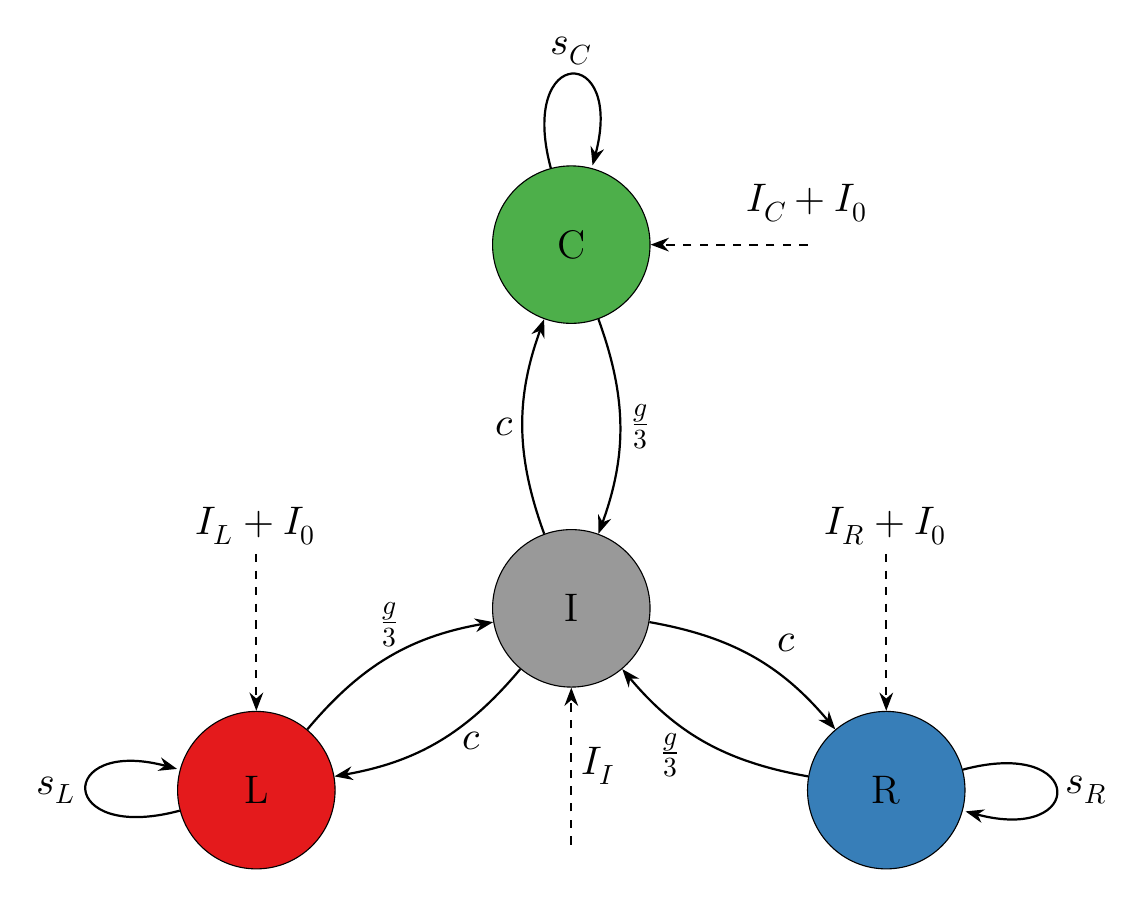
\begin{tikzpicture}[>=Stealth,
  neuron/.style={draw, circle, minimum size=2.0cm, inner sep=4pt, font=\Large},
  arrowlabel/.style={draw=none, fill=none, font=\Large}]

  % Define positions for the excitatory neurons (L, C, R)
  \node[neuron, fill=cb1] (L) at (-4,0) {L};
  \node[neuron, fill=cb2] (C) at (0,6.928) {C};
  \node[neuron, fill=cb3] (R) at (4,0) {R};
  
  % The inhibitory neuron (I)
  \node[neuron, fill=cb4] (I) at (0,2.309) {I};

  % Self-loops
  \draw[->, thick] (L) edge[loop left] node[arrowlabel, left] {$s_L$} (L);
  \draw[->, thick] (C) edge[loop above] node[arrowlabel, above] {$s_C$} (C);
  \draw[->, thick] (R) edge[loop right] node[arrowlabel, right] {$s_R$} (R);

  % E → I connections
  \draw[->, thick, bend left=20] (L) edge node[arrowlabel, above] {$\tfrac{g}{3}$} (I);
  \draw[->, thick, bend left=20] (C) edge node[arrowlabel, right] {$\tfrac{g}{3}$} (I);
  \draw[->, thick, bend left=20] (R) edge node[arrowlabel, left, xshift = -5pt, yshift = -5pt] {$\tfrac{g}{3}$} (I);

  % I → E feedback
  \draw[->, thick, bend left=20] (I) edge node[arrowlabel, right, xshift = 5pt] {$c$} (L);
  \draw[->, thick, bend left=20] (I) edge node[arrowlabel, left] {$c$} (C);
  \draw[->, thick, bend left=20] (I) edge node[arrowlabel, right, xshift = 5pt, yshift = 5pt] {$c$} (R);

  % External inputs (dashed)
  \draw[->, dashed, thick] ($(L)+(0,3)$) -- (L) node[arrowlabel, pos = 0, yshift = 10pt ] {$I_L+I_0$};
  \draw[->, dashed, thick] ($(C)+(3,0)$) -- (C) node[arrowlabel, pos = 0, yshift = 15pt] {$I_C+I_0$};
  \draw[->, dashed, thick] ($(R)+(0,3)$) -- (R) node[arrowlabel, pos = 0, yshift = 10pt ]  {$I_R+I_0$};
  \draw[->, dashed, thick] ($(I)+(0,-3)$) -- (I) node[arrowlabel, midway, right] {$I_I$};

\end{tikzpicture}

\end{document}
